\documentclass[10pt]{beamer}


\usepackage[utf8]{inputenc}
\usetheme{metropolis}
\usepackage{appendixnumberbeamer}
\usepackage[defaultsans]{droidsans}

\usepackage{wrapfig}
\usepackage{tikz}
\usetikzlibrary{positioning}
\usepackage{fancyvrb}
\usepackage{booktabs}
\usepackage[scale=2]{ccicons}

\usepackage{xparse}

\usepackage{xspace}
\newcommand{\themename}{\textbf{\textsc{metropolis}}\xspace}

\usepackage{array}


\title{Mahalanobis-average \\Hierarchical Clustering Analysis \\accelerated on GPU}
%\subtitle{Defence}
\author{Bc. Adam Šmelko}
\date{Supervisor: RNDr. Miroslav Kratochvíl}
\institute{Department of Software Engineering}
\titlegraphic{\hfill
\includegraphics[height=2cm]{img/logo}}

\begin{document}

\maketitle


\begin{frame}{Mahalanobis distance}
	
	Measures a distance between a point and a distribution of points.
	
	\begin{figure}
		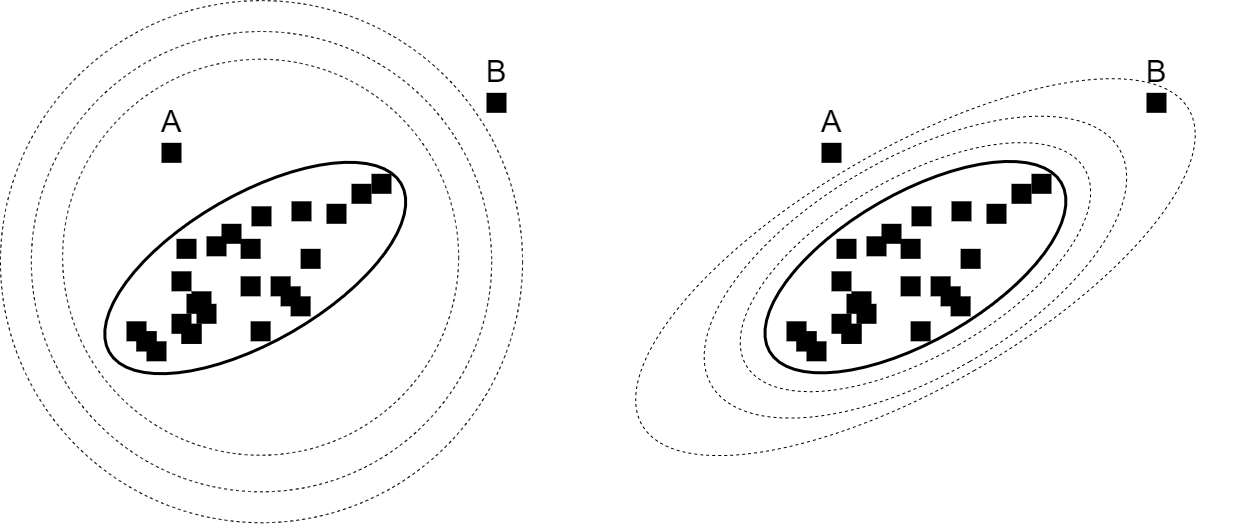
\includegraphics[width=7cm]{img/maha_dist}
	\end{figure}

	Computes the covariance matrix of a distribution which re-scales the axes.
		
\end{frame}


\begin{frame}{Mahalanobis-average clustering}
	
	\begin{itemize}
		\item Originally developed by Fišer et al. for the purpose of monitoring
	minimal residual disease in patients with leukemia.
	\item Captures elliptic clusters that are formed naturally.
	
	\begin{figure}
		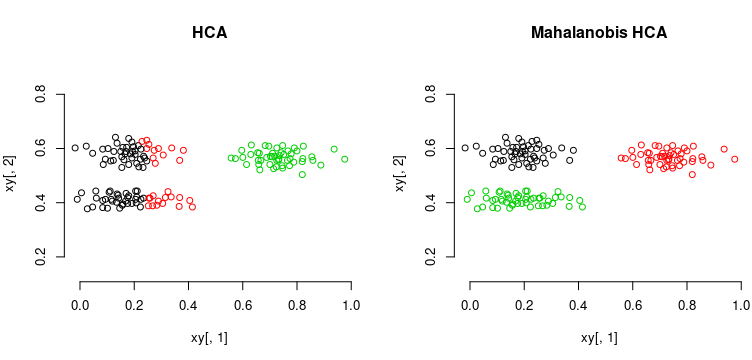
\includegraphics[width=7cm]{img/mhca}
	\end{figure}
	\item Extremely suitable for single-cell cytometry datasets.
	
	\end{itemize}
	
\end{frame}

\begin{frame}{Motivation}
	\begin{itemize}
		\item The Mahalanobis clustering is seriously restricted by performance and complexity to \textbf{$\pm$100K} cells on a common hardware.
	
		\item Modern cytometers produce datasets of \textbf{several million} cells~\dots
	\end{itemize}
	\begin{figure}
	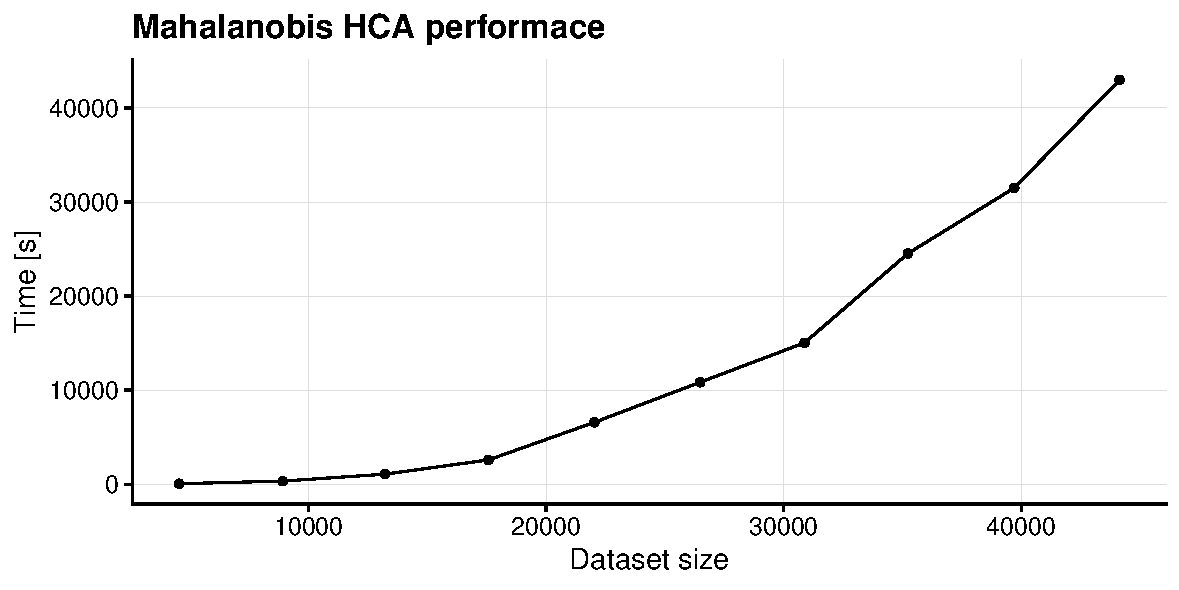
\includegraphics[width=8cm]{img/scalability}
	\end{figure}

\end{frame}

\begin{frame}{Challenges}
	
	Design an implementation of the Mahalanobis clustering that optimizes:
	\begin{itemize}
		\item \textbf{Performance}
		
		Solved by utilizing computing power of a GPU device.
		\item \textbf{Huge input size}
		
		Quadratic space complexity is sub-optimal because the algorithm needs to cluster millions of points.
	\end{itemize}
	
\end{frame}

\begin{frame}{Results summary}
	
	Performance increase:
	\begin{itemize}
		\item 60\texttimes\ to 5000\texttimes\ for single-point datasets.
		\item 8\texttimes\ to 20\texttimes\ for datasets with apriori clusters.
	\end{itemize}

	Reduction of quadratic space complexity to linear; no dissimilarity measurements are stored.
	
	Test machine: Intel Xeon Silver 4110, 256 GB
	RAM, NVIDIA Tesla V100 PCIe 16 GB
	
\end{frame}

\begin{frame}{Results summary}
	
	\begin{tabular}{cc}
		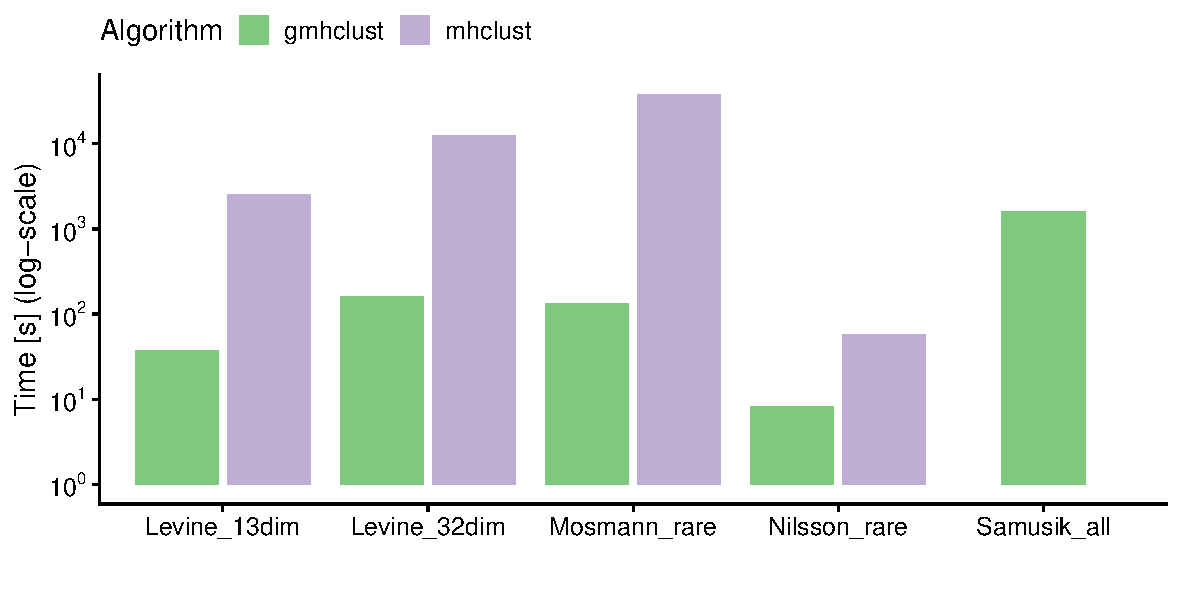
\includegraphics[width=6cm]{../img/mixed_perf_comp} & 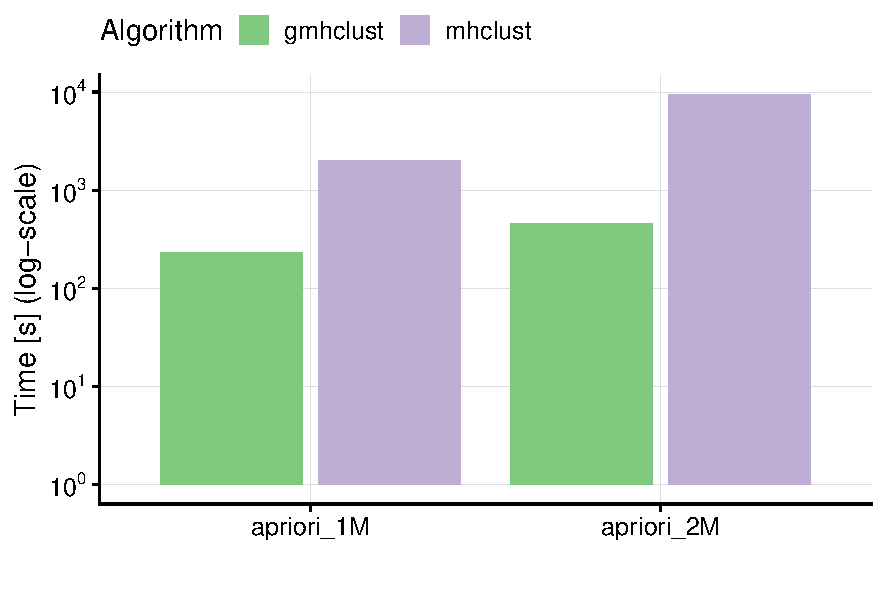
\includegraphics[width=4.4cm]{../img/apriori_perf_comp} \\
	\end{tabular}
	\begin{figure}
		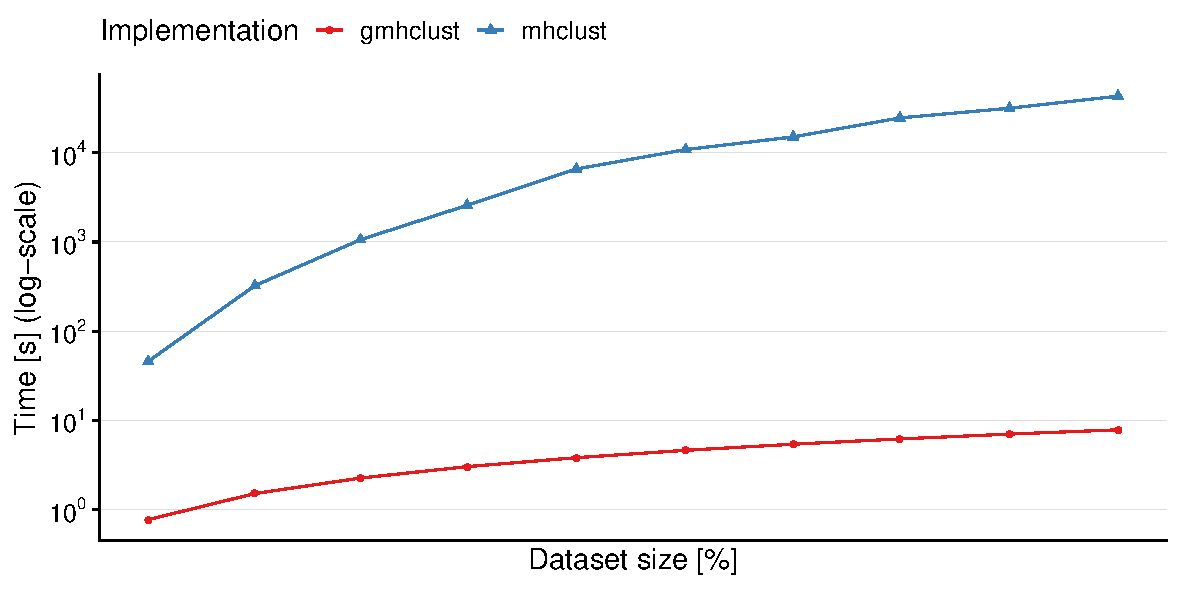
\includegraphics[width=7cm]{../img/single_perf_comp}
	\end{figure}
	
\end{frame}

\begin{frame}{Results comparison}
	
	\begin{block}{Clusterings comparisons of single-point dataset}
		
		\begin{columns}
			\column{\linewidth-7cm}
			
			Generally similar
			
			\column{7cm}
			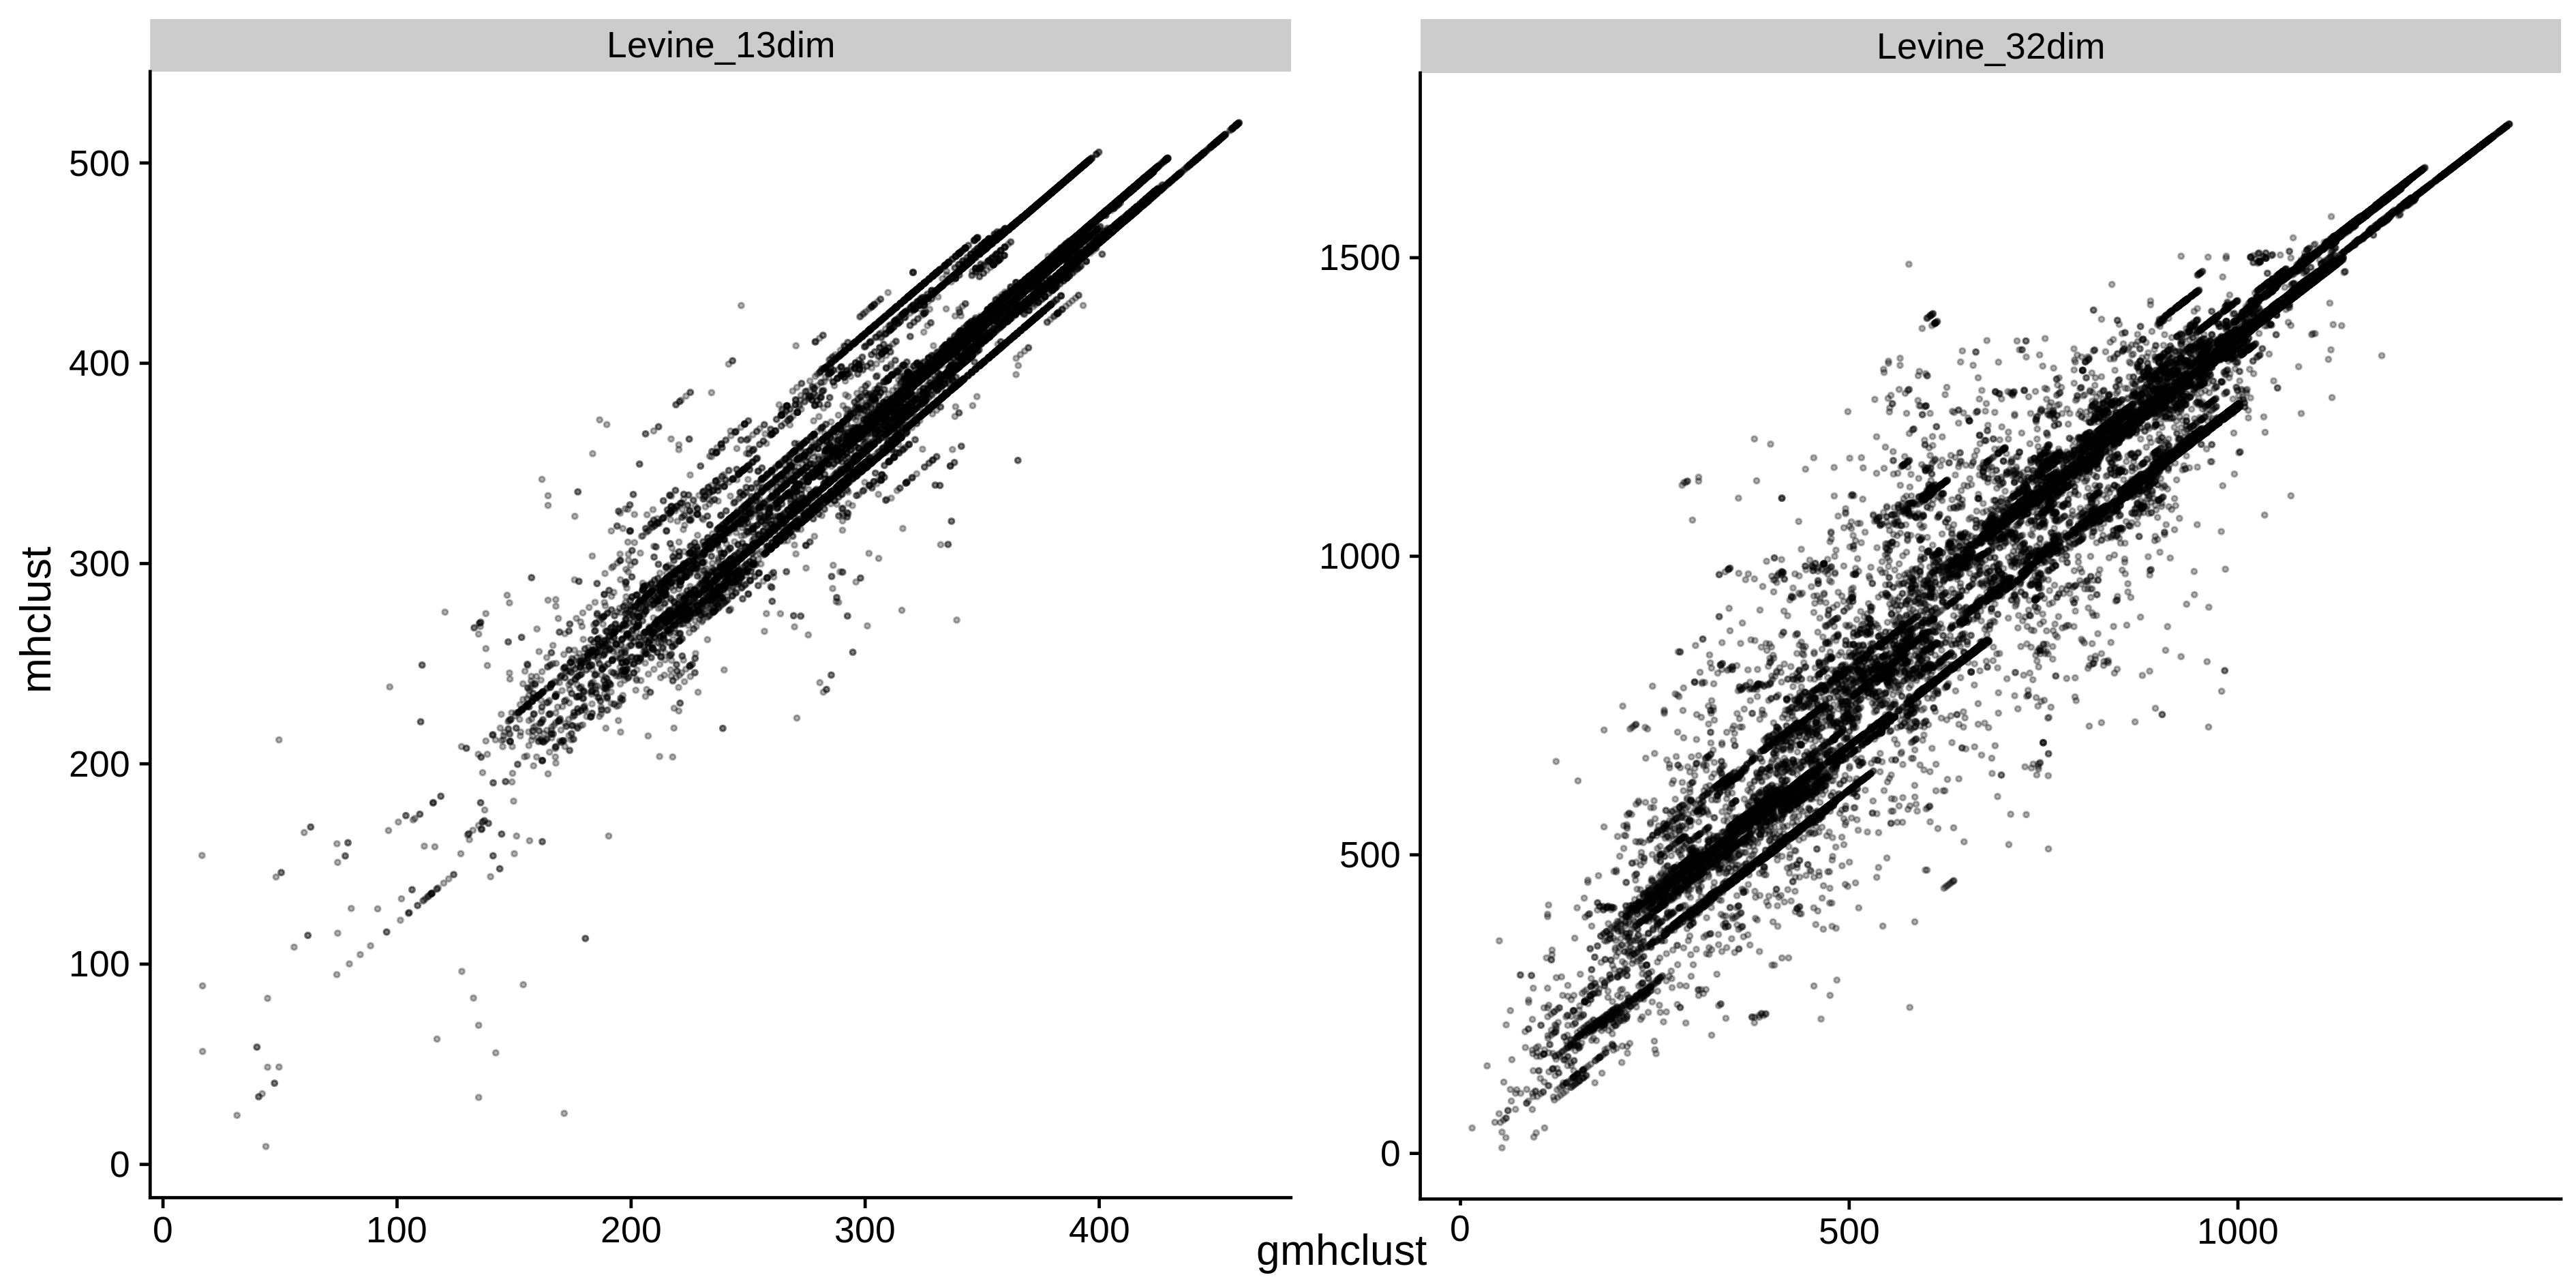
\includegraphics[width=7cm]{img/single_result}
			
		\end{columns}
	\end{block}
	
	\begin{block}{Clusterings comparisons of datasets with apriori clusters}
		\begin{columns}
			\column{\linewidth-7cm}
			
			
			Practically no difference
			
			\column{7cm}
			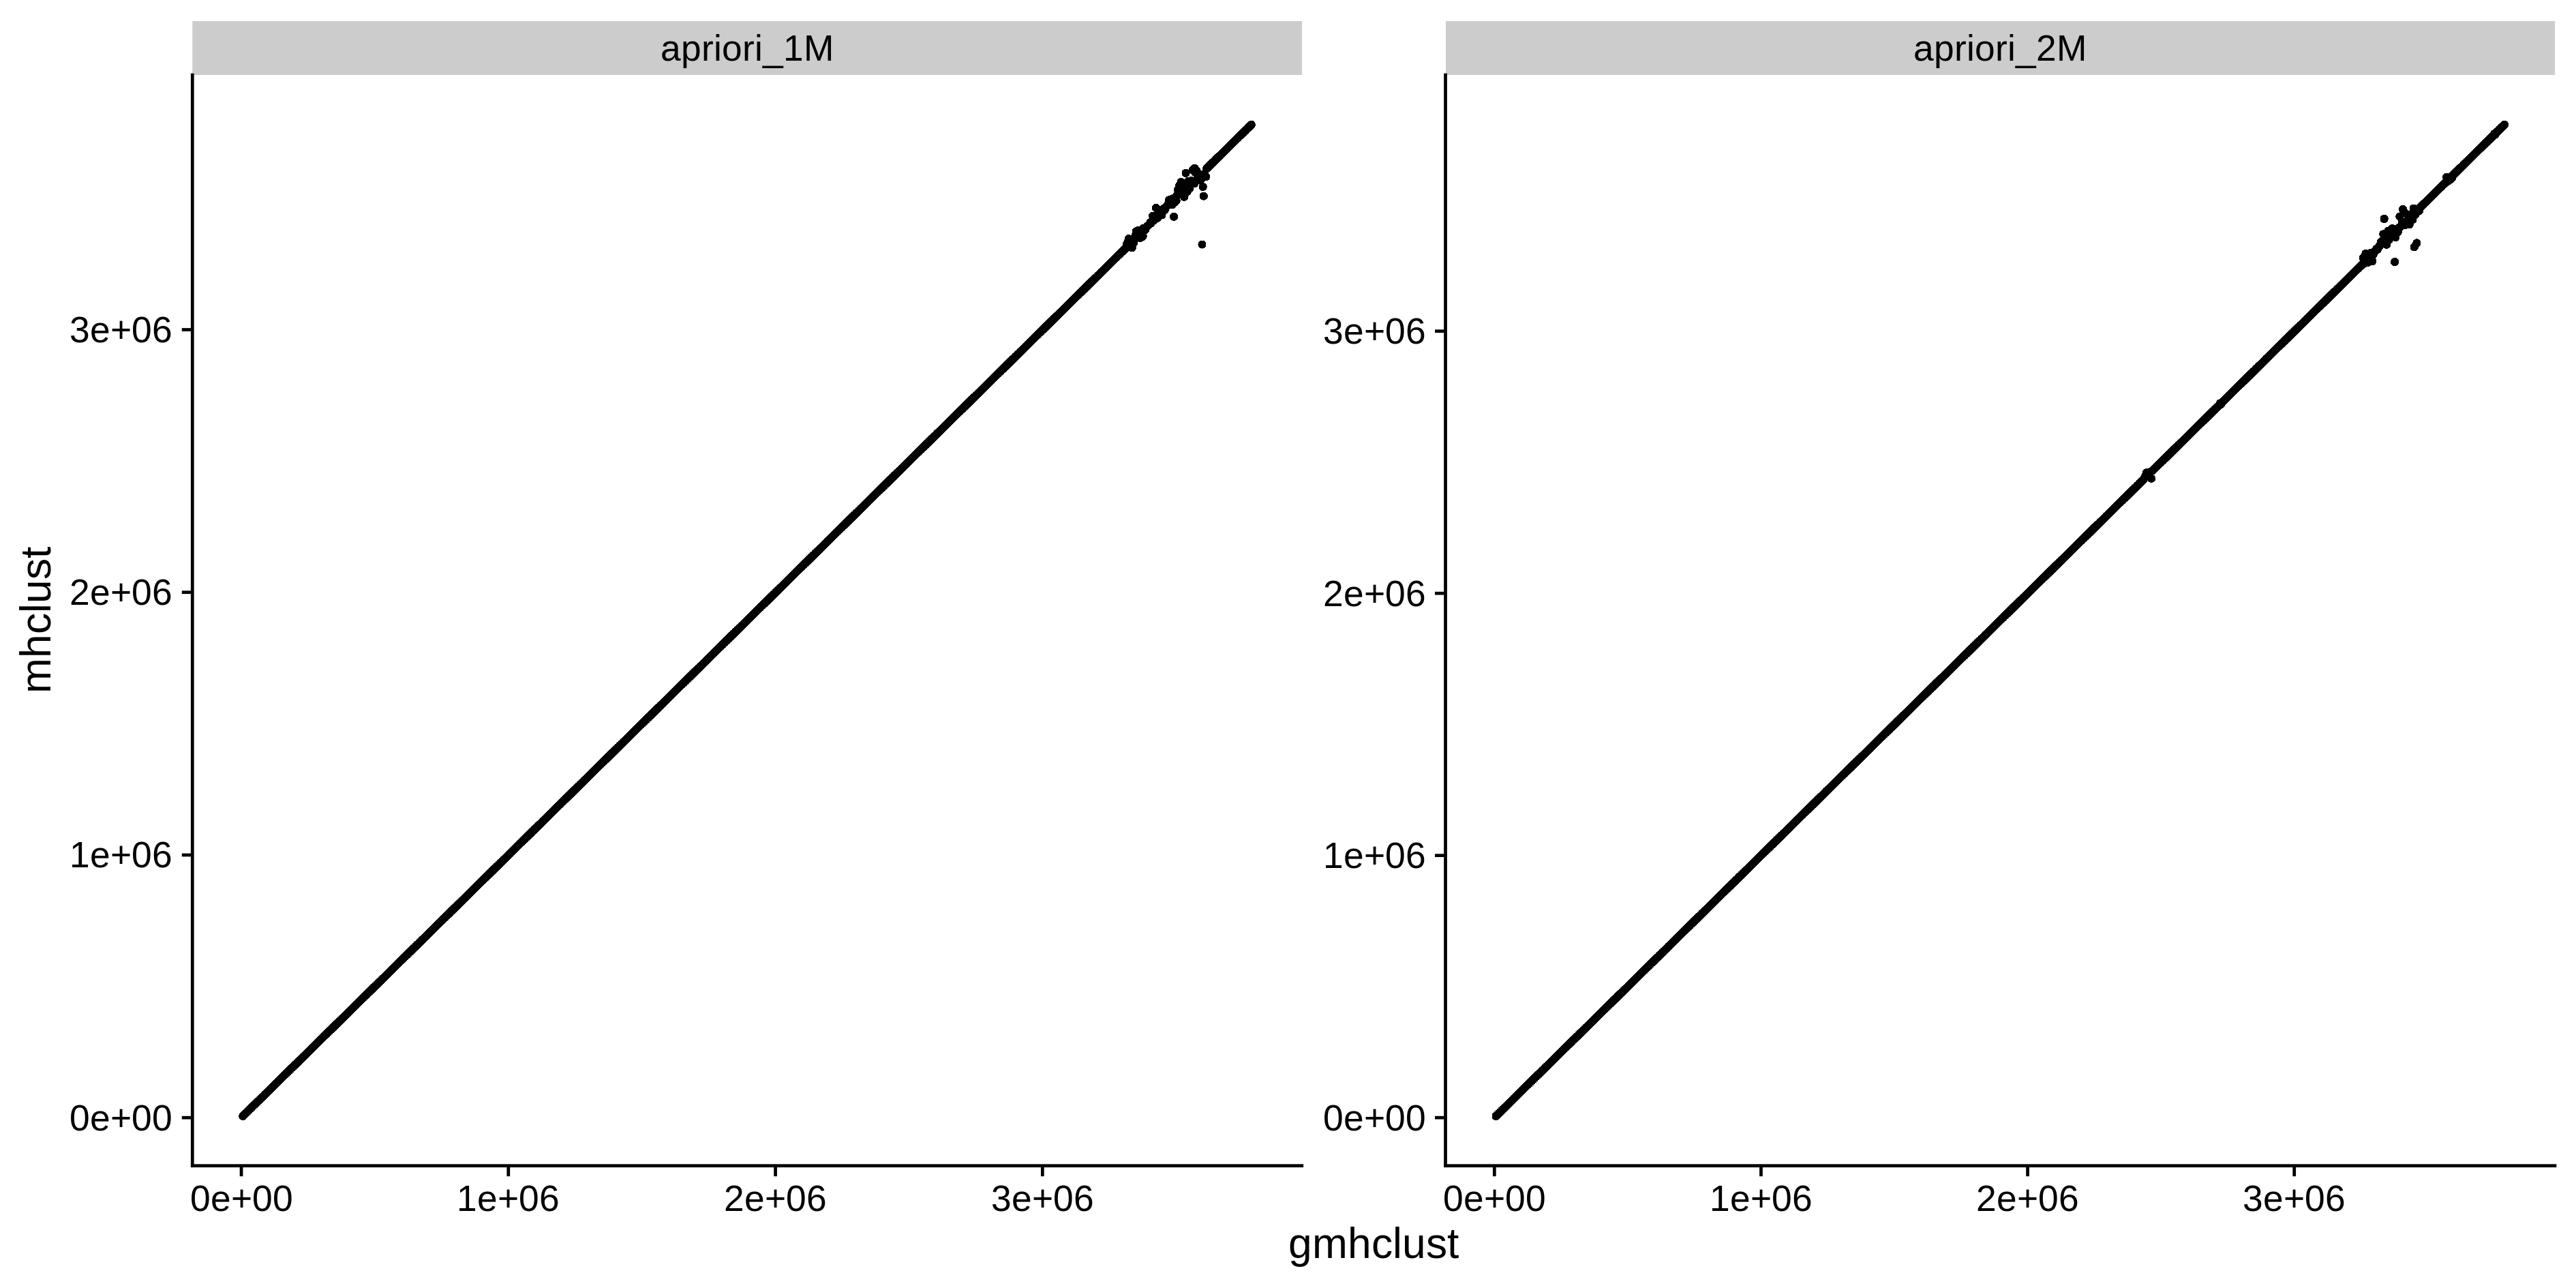
\includegraphics[width=7cm]{../img/apriori_result}
			
		\end{columns}
	\end{block}
	
\end{frame}


\begin{frame}{Implementation details}
	
	The main principles:
	\begin{itemize}
		\item Data continuity
		\begin{figure}
			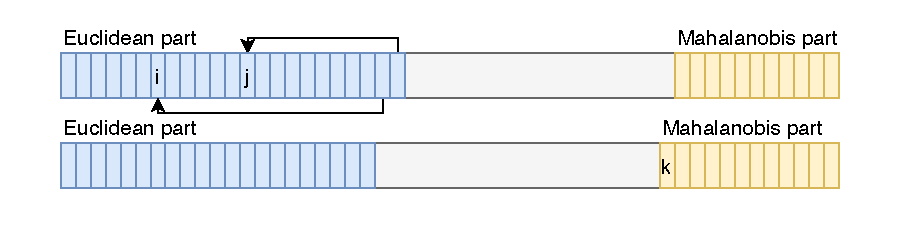
\includegraphics[width=8cm]{../img/data}
		\end{figure}
		
		\item Task-specific CUDA kernels
		\begin{itemize}
			\item \texttt{update\_eucl}
			\item \texttt{update\_maha}
			\item \texttt{compute\_centroid}
			\item \dots
		\end{itemize}
	\end{itemize}

\end{frame}

\begin{frame}{Implementation details}
	
	Used HCA variant: \emph{Nearest neighbor HCA}
	\begin{itemize}
		\item $\mathcal{O}(u\cdot n^2)$ time complexity using linear space where $u$ is the upper bound for the number of clusters to update each iteration (the worst case $\mathcal{O}(n^3)$).
		\item The number of cached closest neighbors can be tweaked.
	\end{itemize}

	\begin{figure}
		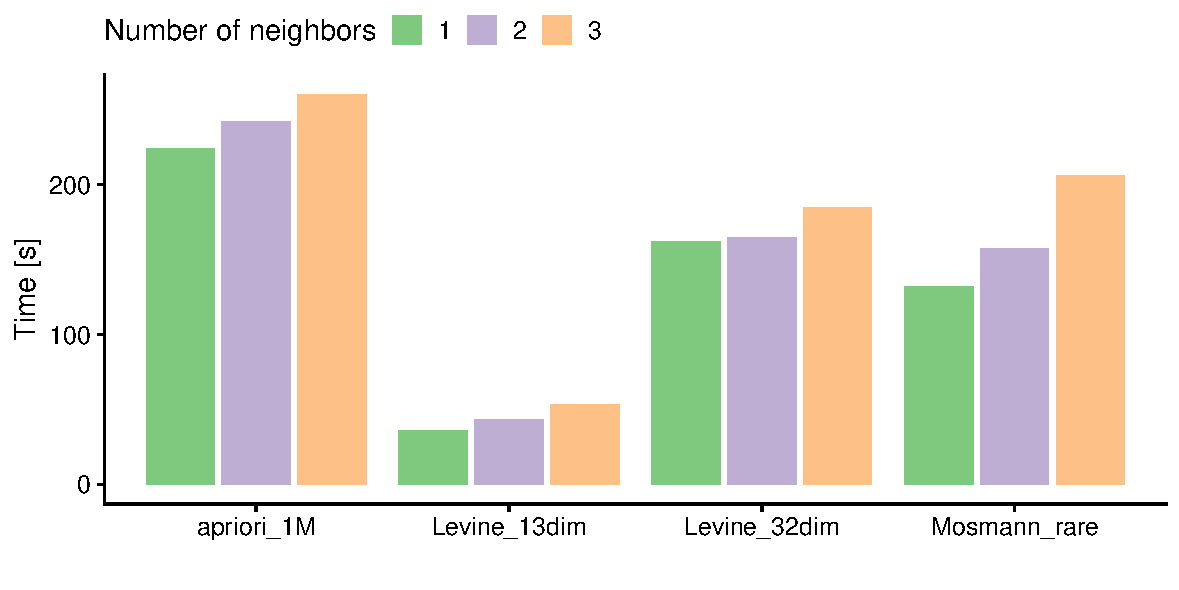
\includegraphics[width=7cm]{../img/neighbor_compare}
	\end{figure}
	
\end{frame}

\begin{frame}{Future work}
	
	Future work: 
	\begin{itemize}
		\item Improve the dissimilarity measure for a better clustering
		of small clusters.
		\item Improve parallelism in presence of apriori clusters.
		\item Switch to \emph{Dissimilarity matrix HCA} when a small amount of clusters remains.
	\end{itemize}
	
\end{frame}

\begin{frame}{Conclusion}
	
	\begin{itemize}
		\item Novel implementation of the Mahalanobis clustering algorithm on GPU.
		\item Speedup up to 5000\texttimes\ on practical datasets.
		\item MHCA performance now practical for common datasets with millions of data points.
	\end{itemize}
	
\end{frame}

\begin{frame}[standout]
	
  Thank you for attention.

\end{frame}


\end{document}